\documentclass{standalone}

\usepackage{tikz}
\usetikzlibrary{positioning, arrows.meta}

\newcommand{\op}[2]{
  \node (#1) [draw, circle, #2] {$o_{#1}$};
}

%
%   1 2
% 0 3 5
%   4 
%

\begin{document}
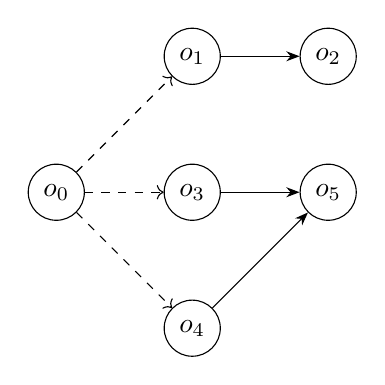
\begin{tikzpicture}[ve/.style = {dashed, ->},
    hb/.style = {>=Stealth, ->}]
  \op{0}{};
  \op{3}{right = of 0}  \op{5}{right = of 3}
  \op{1}{above = of 3}  \op{2}{right = of 1}
  \op{4}{below = of 3}

  \path (0) edge[ve] (1)
	    edge[ve] (3)
	    edge[ve] (4)
	(1) edge[hb] (2)
	(3) edge[hb] (5)
	(4) edge[hb] (5);
\end{tikzpicture}
\end{document}